\documentclass[pdftex,12pt,a4paper]{report} 

% Document settings

\usepackage{fullpage}
\usepackage{cite}
\usepackage{datetime} 
\usepackage{geometry}
\usepackage[pdftex]{graphicx}
\usepackage{verbatim}
\usepackage{todonotes}

\geometry{verbose,lmargin=3cm,rmargin=3cm}

\newcommand{\HRule}{\rule{\linewidth}{0.5mm}}

\begin{document}

%--------------------------------------------------------------------------------

% Title page of report

\begin{titlepage}

\begin{center}

% Upper part of the page
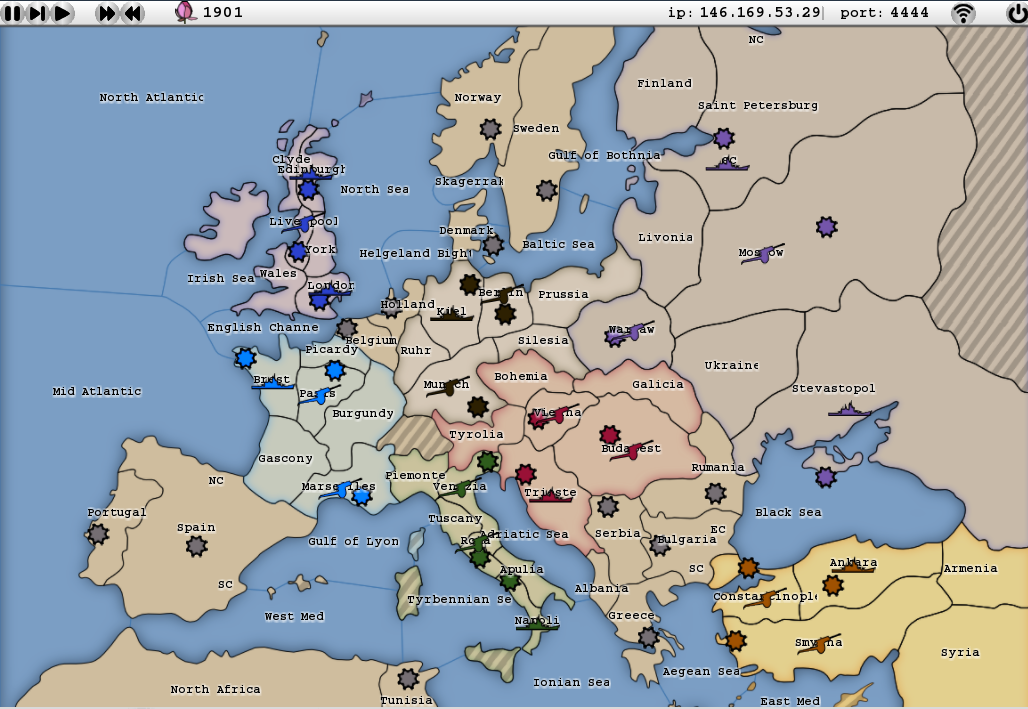
\includegraphics[width=0.60\textwidth]{./screenshots/StartMap.png}\\[1cm]    

\textsc{\LARGE Imperial College London}\\[1.5cm]

\textsc{\Large 3rd year group project}\\[0.5cm]

% Title
\HRule \\[0.4cm]
{ \huge \bfseries Automated negotiation in the game of Diplomacy}\\[0.4cm]

\HRule \\[1.5cm]

% Author and supervisor
\begin{minipage}{0.4\textwidth}
\begin{flushleft} \large
\emph{Author:}\\
Luca \textsc{Deltodesco} \\
Matthias \textsc{Hueser} \\
Andras \textsc{Slemmer} \\
Cliff \textsc{Sun} \\
Luke \textsc{Tomlin} \\
\end{flushleft}
\end{minipage}
\begin{minipage}{0.4\textwidth}
\begin{flushright} \large
\emph{Supervisor:} \\
Dr.~Iain \textsc{Philipps}
\end{flushright}
\end{minipage}

\vfill

% Bottom of the page
{\large \today}

\end{center}

\end{titlepage}


%--------------------------------------------------------------------------------

\begin{abstract}

In this project we created a negotiation-capable AI framework for the
game of 'Diplomacy'. On the tactics-side a pattern-weight learning
algorithm \cite{Shapiro02} coupled with a best-first search strategy
finder is used. In addition a DAIDE-conforming \cite{DaideWeb} subsystem
comprising GUI client and server was implemented. To our knowledge our server
is the first implementation using the functional language Haskell. Finally
we conducted various games of humans against AI bots to estimate the playing
strength of our bot. We are optimistic that our findings can be related to
the general research field of \textit{Automated negotiation}. Our GUI client is
novel in the way that it can be deployed as a native application, web and 
smart-phone.

\end{abstract}

\setcounter{tocdepth}{2} % Set the depth of toc indexing

\tableofcontents

\pagebreak

%--------------------------------------------------------------------------------

% Set arabic numbering for auto-indexing

\renewcommand*\thesection{\arabic{section}}

\section{Acknowledgements}

We thank our supervisor Dr. Iain Philipps (iccp@doc.ic.ac.uk) for his
support and guidance throughout the duration of the project. For the
software engineering aspects of the project Robert Chatley's course
'Software Engineering Methods' was very instructive, improving our
process and team collaboration. \\

Also we would like to direct our thanks at the whole DAIDE community
giving us an environment to test our AI bots. \\

The programming languages that were used for server and GUI client
have come a long way in recent years. Without the dedication of the
\textit{Haskell} and \textit{HaXe} communities to provide easy-to-use
libraries it would not have been possible to make progress on 
several fronts at the same time.

\pagebreak

%--------------------------------------------------------------------------------

\section{Group members} 
Luke Tomlin (Team leader) \\ 
Luca Deltodesco ld509@doc.ic.ac.uk \\ 
Matthias Hueser mh2308@doc.ic.ac.uk \\
Andras Slemmer as13609@doc.ic.ac.uk \\
Cliff Sun chs09@doc.ic.ac.uk \\

%--------------------------------------------------------------------------------

\pagebreak

\chapter{Introduction}

\section{Automated negotiation}

Automated negotiation is a field of increasing interest in political
strategy, psychology and economics. At the small scale each human 
is concerned with negotiation: from families to businesses one can always
discern the common pattern of autonomous agents trying to reach some joint goal. 
Another instance of \textit{cooperating agents} have been studied recently
in the field of \textit{Distributed artificial intelligence}: Grosz et al
looked at ``Collaborative plans for complex group activities'' \cite{Grosz96}
whereas issues of consensus-finding has been a focus of \textit{Distributed computing}
for a long time. \\

The military applications of ``Automated negotiation'' generally assume a number
of \textit{non-cooperating} agents playing an \textit{adversial game}. The field
of classical game-theory grew out of the need to analyze such situations.
While successful it is doubted whether its premise of purely rational entities
can be justified in reality. It is universally accepted that a lot of actions
are driven by irrational instincts rather than deliberate planning. The question
remains whether ``Automated negotiation'' theory should try to imitate humans
or overcome their alleged ``weaknesses''. If the first approach is taken issues
of \textit{Emotion modelling} and \textit{Relationship inference} need to 
be addressed and a proper representation found. \\

\section{Diplomacy and negotiation}

In this context the \textit{Game of Diplomacy} is an ideal test-bed 
to explore various paradigms of ``Automated negotiation''. This is because
a number of its features can be directly related to the complex, unpredictable
domains encountered in reality: 

\paragraph{Zero-sum property}
A game is said to be \textit{zero-sum} if one's player gains are another
player's losses. This is clearly the case in Diplomacy where an advance
into a favourable board position inevitably results in a another power's
unit being dislodged from this position. In reality resource- or
military conflicts behave in the same way.

\paragraph{Imperfect information}
There are two levels of uncertainty in Diplomacy: On the one hand all move
orders are written down secretly and then revealed simultaneously during
the move resolution phase. So a power has no way to plan with the moves 
of its opponents but instead has to resort to ``move prediction''. It
is obvious that almost every adversial game encountered in reality
shares this property. Negotiation itself is another
layer of uncertainty in Diplomacy: messages are normally not 
posted publicly and hence no player can know in advance which
strategies its opponents discussing.

\paragraph{Simultaneous movements} 
Simultaneous moves are an important element of Diplomacy's game-play
and contrast with classical turn-based games like Chess or 
Backgammon. They give the game a dynamic, real-time flavour -- 
in reality actions happen -- if not all at once but certainly
not in a pre-determined turn order.

\paragraph{Deterministic operators}
Apart from the initial assignments of players to powers there
is no element of chance in Diplomacy. In reality many domains
can be modelled in this way once a bot has compiled its ground
rules in a knowledge base.

\subsection{Rationale of negotiation}

Besides the necessity to create effective long-term strategies
negotiation is integral to the game-experience of Diplomacy.
Consider a solitary power trying to open several war-fronts
at the same time. This strategy is bound for doom because 
the other negotiating agents will quickly forge a coalition
against the loner. Negotiation is also advantageous in that

\pagebreak

\section{DAIDE framework}

There is a thriving internet-based community around the Game of
Diplomacy \cite{DipArchive04} \cite{DipPouch04}. A welcome effect
is that amateur players have access to a rich body of strategic
knowledge which forms the basis of many existing bots. Until the
90s bot development has been ad-hoc and it has been difficult
to find a common platform to validate their playing strength. To remedy
this the DAIDE framework \cite{Daide04} has been created. It comprises
a language specification for client-server interaction \cite{DAIDEsyntax10}
 \& negotiation and various useful tools: 

\begin{itemize}

\item The \textit{DAIDE Server} enables both human and AI players to
      compete in a game. A screenshot of the Main GUI is given below:

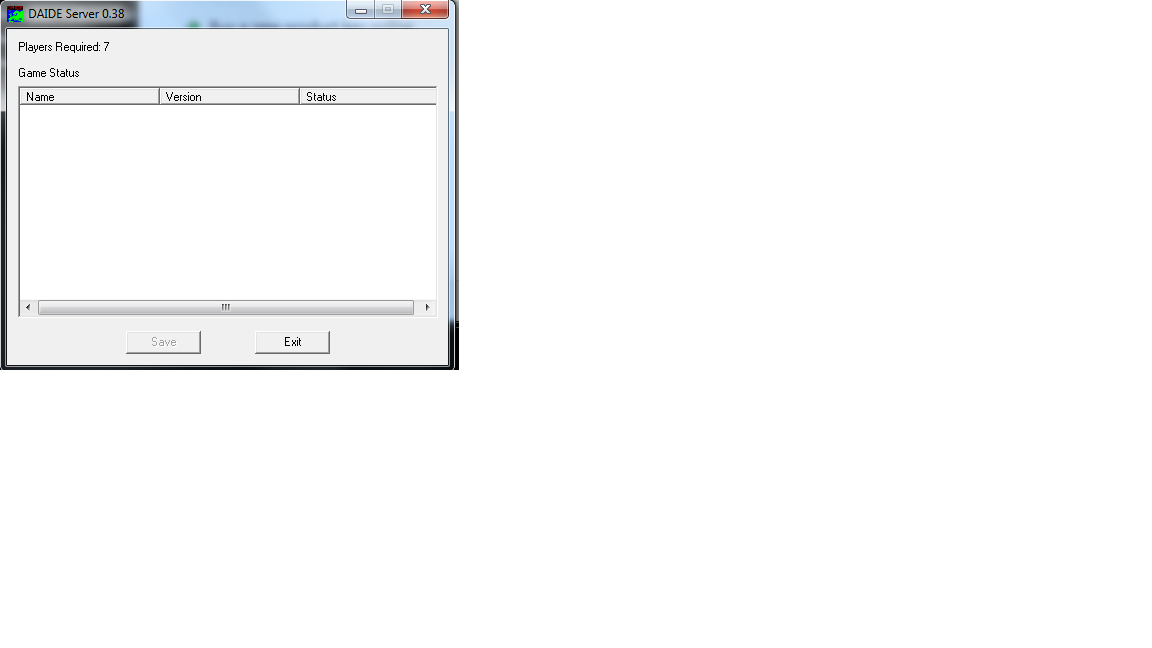
\includegraphics{./images/DAIDEServer.png}

\item \textit{DAIDE Mapper} is a server hook-in to visualize
      the game state.


\todo{Find a screenshot of the DAIDE mapper}

% \includegraphics[width=0.60\textwidth]{./images/DAIDEMapper.png}

\end{itemize}


 and many AI
players, so called bots, have been created in the past. Most of the
existing AI players are quite effective decision-makers in general but
few of them support negotiation or reasoning about the relationship of
the powers in the game. Our project aims to create a framework for
Diplomacy, including a GUI client, a game server and a collection of
bots. The highest evolution of our series of bots should be able to
analyze and act upon messages of human / AI players and issue messages
to other players. In particular we aim to unify negotiation and
general strategy, given that negotiation is simply 
cooperative decision-making and only a layer of communication and
trust models have to be added. \\

Finally experiments are conducted to determine whether there is a
reward associated with negotation capabilities. This required careful
study and implementation of automated negotiation techniques from
other domains in AI / Game Theory. Thus the project gave us ample
opportunity to be creative and test different approaches using the
DAIDE-conforming game framework also produced for the project. DAIDE
is a standard client-server protocol \cite{DaideWeb} which serves as a
'common language' for different Diplomacy bot implementations,
enabling them to play a game together on a conforming server. We
explain the concepts of \textit{press levels} in a specific section on
\textit{DAIDE}.

%--------------------------------------------------------------------------------

\pagebreak

\chapter{The game of Diplomacy}

Only the concepts of the game necessary to understand the 
algorithms of the AI / negotiation are described here. For a
definitive reference of the game rules refer to \cite{DiploRules00}.

\section{Overview}

The Game of Diplomacy is a round-based multiplayer strategy-game set
in WWI Europe. It was conceived by Alan Callhamer in 1954. Besides
the joy it has brought to players he designed it to see how 
secret negotiations affect strategy games. Each player controls a 
European power which initially operates from a set of supply centers.
The objective of the game is to control the majority of supply-centers
on the map, using army movements to conquer new bases and ultimately
eliminate all opponents from the map. There are alternative winning
and draw conditions -- such as a simple majority after a time limit -- 
but we have not considered them in our project.

\paragraph{Game elements}

The game board consists of 73 provinces. Half of them are 
called \textit{supply centres}.

\paragraph{Provinces}

There are three type of provinces: Water, land and coastal 
provinces. In general the adjacencies of provinces are obvious
from the game map; in some intricate cases the rulebook needs to
be consulted. Each province can optionally be occupied by one
unit of the correct type.

\paragraph{Supply centres}

A subset of the land provinces are supply centres which can be 
occupied by a power's unit. At the end of the season each power
can build additional units in its non-occupied supply-centres.
This happens in the context of an important constraint: A power 
can never more units than supply centres controlled at the end
of each year. Both are reconciled in the build / retreat phases
at the end of each year: If there is an overhead of units they
have to be dislodged.

\paragraph{Units}

There are two type of units -- Armies and fleets -- controlled
by a power. Each can only move to provinces of the correct type.
Fleets can occupy water and coastal provinces, whereas armies 
move on land.

\section{Game turns / phases}

A game is divived into a number of turns, which is either a
\textit{fall turn} or a \textit{spring turn}. Two turns comprise
a year, the first one being 1901. Each turn contains a number of 
\textit{phases} in which the players negotiate, formulate
their orders and submit them to the server. The order of action in
fall and spring terms are the same, except that only the fall term
has a \textit{gaining-and-losing} phase.

\paragraph{Diplomacy phase}
In this phase players jointly devise strategies, forge alliances and
suggest move orders for the next round. Conversations can be 
one-to-one or in groups. None of the agreements
reached are binding and can even be used to deliberately 
mislead another player and prepare a back-stab. Lastly it is possible
to broadcast announcements to all players.

\paragraph{Order writing phase}
Afterwards each player writes down orders for its units and prepares
them for submission for the game server. There is no communication 
between players in this phase. 

\paragraph{Order resolution phase}
At this stage all orders are simultaneously revealed to the server,
who announces them publicly. Now the effects of the moves on the
map state are determined, resolving them according to the game rules.
In simple cases only standoffs between different move orders need
to be considered but the complex game rules result in many special
cases that need to be considered by the server. 

\paragraph{Retreat and Disbanding phase}
The effects of the submitted orders might make it necessary to retreat
some units from its current provinces. The only choice given to a
players is the destination province of a retreat which needs to
adjacent to the province from which the unit has been dislodged. Once
these are selected a set of \textit{retreat} orders is created and
resolved immediately by the server. As for ordinary moves standoffs
between retreat orders can occur; in this case each unit involved in
such a standoff is immediately \textit{disbanded} from the map. The
same happens if a player does not give a destination for a unit that
has to retreat.

\paragraph{Gaining and Losing phase}
As mentioned initially this phase only occurs in a \textit{fall turn}.
The purpose of this phase is to adjust the number of units of a power
to the number of supply centres it controls, reflecting its current
strength. Players can submit build and disband orders as explained
below. 

\section{Order submission}

The submission of orders happens \textit{simultaneously}; the game
rules also stipulate that all orders are publicly announced. The diplomacy
phase of a game turn allows powers to signal their actual intention or
mislead other powers about them. In addition to revealing their move
orders powers can also forge alliances and devise strategies
collectively. Ultimately there is no limit to the scope of negotation
messages.

\section{Order types}

In the \textit{order writing} phase each power can optionally submit
an order for each unit controlled. Not specifying an order for a 
unit is interpreted as a \textit{hold order}. 

\paragraph{Hold order}
A unit receiving a hold order does nothing and keeps a unit on its 
current location. 

\paragraph{Move or attack order} 
Move orders shift units from their original position to one of its
adjacent provinces. A move can either be successful, result in a
standoff or fail because of insufficient strength. 

[1cm]
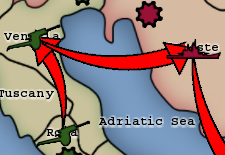
\includegraphics{./screenshots/Move0.png} % OK Move
[1cm]
The red arrows indicate that the move order succeeded and the units
will be moved to the destination. In general a move order succeeds
if the attacking party has higher strength than the defense. Each 
support order increases the strength of offense / defense by 1.

[1cm]
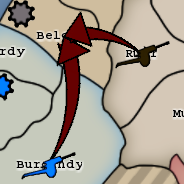
\includegraphics{./screenshots/BouncedMove.png} % Standoff
[1cm]
The dark-red arrows indicate that the move bounced and the units will
remain in the same place. This is because both units are attempting 
to move to the same location and have the same strength, none being
supported by another unit.

\paragraph{Support order}
A support order assists another unit's move or hold order. It can either be
used defensively to protect a province against an attack order or increase
the odds of another unit conquering a province. 

[1cm]
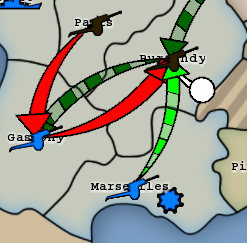
\includegraphics{./screenshots/DefRetreat0.png}
[1cm]
Here the French unit at Marseille is supporting the move of it's comrade at
Gascony to Burgundy. The German unit at Burgundy was attempting to support
the move of it's ally at Parise to Gascony. In the end  it's support was
cut by a dislodgement from the French unit. After the moves are resolved, 
the Burgundy unit will be dislodged at the white marker and forced to 
attempt a retreat in the next phase.

\paragraph{Convoy order}
This order type is restricted to fleet units. They allow to transport
an allied army between two coastal provinces across the water. In general
such convoys can be chained: If an army tries to move along a path of
several water provinces all of those need to be \textit{convoyed} 
by a fleet.

\paragraph{Retreat order}
A retreat order normally only occurs in the retreat / disband phases of the
fall and spring terms. If a unit is overpowered by an attack on its
province it needs to move to an adjacent province. The exact destination
is specified by the player in a retreat order.

[1cm]
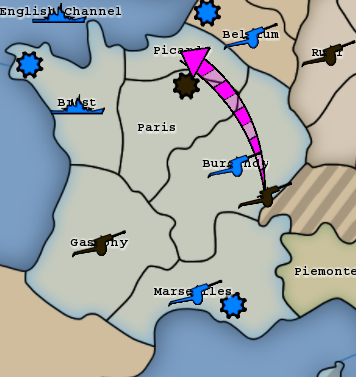
\includegraphics{./screenshots/DefRetreat2.png}
[1cm]
Here the German unit previously dislodged from Burgundy has succesfully retreated to Picardy. 
It is possible although quite rare for a retreat order to fail (Perhaps due to two dislodged
units attempting to retreat to the same space) and in such case the unit would be removed from the map.

\paragraph{Disband order}
If a unit cannot perform a retreat then the unit is removed from the map automatically.

[1cm]
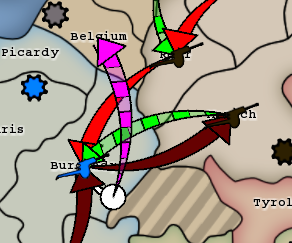
\includegraphics{./screenshots/ImmRetreat0.png}
[1cm]

\paragraph{Build order}
This order is limited to the \textit{Gaining and losing phase} where unit numbers
are reconciled with supply centre control. At the end of each year the
server signals the maximum number of units a player can have in the following
turn. Empty supply centres can now be used to build any surplus units.

\paragraph{Remove order}
Any surplus units that do not have a ``supporting supply centre have to be removed
at the end of the year. With \textit{Remove orders} the player can select which
units should be removed from the board.

\paragraph{Remove / dislodge order}


%--------------------------------------------------------------------------------

\pagebreak

\section{Related work}

\subsection{Existing negotiation bots}

\paragraph{Diplomat by Kraus et al}

Kraus et al used the multi-agent paradigm to implement the first
Diplomacy bot capable of negotiation \cite{Kraus95}. Their bot
comprises a collection of local agents that are dynamically bound to
different negotiation modules. In analogy to a government they define
a 'Prime Minister', 'Ministry of Defense', 'Foreign office',
'Headquarters' and 'Intelligence' which deal with arbitration,
creating DAIDE messages, long-term strategy formulation and so
forth. Hereby the 'Prime minister' fixes the character traits of the
bot. To maintain information about other players and their intentions
a so-called Knowledge and Belief base is used. For details refer to
\cite{Kraus88}

\paragraph{DipGame testbed by Fabregues}

\paragraph{SeaNail by Lorber}

The SeaNail AI \cite{Lorber98} uses a Dynamic Programming approach to
maximize the number of campaigns matching the current aims of the
bot. For instance if a supply centre is selected for capture and a
certain defense strength is estimated units that overcome this have to
be selected. For every combination of

\paragraph{Previous project by Huff et al}

In a previous group project at Imperial College \cite{Huff05}

\subsection{Strategy-only bots}

There have been various earlier efforts to create a Diplomacy bot
limited to DAIDE press level 0 \cite{DAIDEsyntax10}. While early
approaches used classical AI techniques like Best-First-Search there
has been a move towards multi-agent designs that assign agents to
board units or split the problem domain along different tasks. As
negotiating is the primary goal of the project we are re-using
concepts like temporal difference learning \cite{Levinson94} and the
valuation of provinces \cite{Huff05} to create a strong AI player.

%--------------------------------------------------------------------------------

\pagebreak

\section{Project aims}

High-level requirements were discussed in the initial phase of the
project (weeks 1/2) with our project supervisor. The terms of the
collaboration were such that only certain high-level goals were
defined and decisions about which AI techniques to use were decided once
related research has been explored.

\begin{itemize}

\item The over-arching goal and hence the most critical requirement is
  to design and implement a negotiation bot for Diplomacy whose
  performance is then compared to existing bots in an experimental
  setting. 

\item A collection of other bots which are not capable of communication
  should be created for purposes of comparison. These should use
  proven techniques from the fields of Game Theory and Multi-Agent
  systems, including learning, tactics and long-term strategies. All
  bots should support the DAIDE protocol to compete against existing
  bots on the DAIDE windows server.

\item To facilitate experimentation an open-source framework
  conforming to the existing DAIDE protocol should be created. This
  framework comprises a server which hosts games for automated and
  human clients and a tool to gather game statistics. The imperative
  behind this is to feed-back into the Diplomacy community as a whole,
  providing a multi-platform server (Windows DAIDE server exists) for
  the first time.

\item In addition a framework for simple generation of Diplomacy bots
  is envisioned: Right now a player needs to re-invent the wheel by
  implementing well-established game-tree search techniques or certain
  Machine Learning paradigms in low-level terms. This is clearly
  unsatisfactory. Our framework helps to shift the focus to
  interesting new techniques from academia which can be coded up and
  layered on top of primitives. Actually this framework is used for
  the 2nd objective above to quickly generate a series of bots with
  increasing functionality.  (Abstract client pattern) This also works
  as a proof-of-concept for the server framework. At the users
  convenience extensions are written in the high-level language
  Haskell which is more expressive than C++ and natural to
  practitioners in the field of Artificial Intelligence / Game Theory.

\item Finally to test our server and provide a visually pleasing user
  interface we deliver a DAIDE-conforming GUI client for the Game
  of Diplomacy.  Rather than forcing the player to use a particular
  device all back-ends of the HaXe platform are supported, including
  HTML5/JS, Flash and C++.

\end{itemize}

In the above listing the requirements are decreasing in
importance. Some of the above look indivisible in nature but we have
still managed to extract user-stories to support time-boxed
iterations. Requirements management was two-fold: Each
team-member kept in mind the overall contract with our supervisor (see
above) which defines the direction of the project.  Based on this
User-Stories were defined which guide the primary development focus
during the iterations.

%--------------------------------------------------------------------------------

\pagebreak

\section{Strategy and tactics}

As listed in the \textit{Introduction} section there were previous
attempts of creating a strong AI for Diplomacy: Kraus \cite{Kraus95}
put emphasis on negotiation whereas \cite{Shapiro02} used
\textit{Temporal difference learning} to guide move selections. For
our AI we augment Shapiro's technique with state utility functions
that should lead to more realistic pattern-weights. It is a
common-place in the Diplomacy AI community that game-tree based search
techniques are intractable; The branching factor of one turn
is roughly $6^{n}$ where n is the number of units controlled by a
player. Considering the combinations of moves of all players we get
$2^{91}$ possibilities \cite{Shapiro02}. Thus we did not follow this
path but focussed on \textit{learning} and ad-hoc goal-directed move
formulation. \\

Subsequently we describe the concepts of \textit{move patterns},
\textit{pattern weights} and present our state evaluation functions.

\subsubsection{Move patterns}

A primitive pattern is a property of a move; Examples are its type,
features of its origin \& destination provinces or estimated support
strength. Each \textit{move pattern} is a n-pattern where n is the
number of primitive patterns that a given move matches. Hence as n
increases a pattern goes from the general to the specific and will
match fewer and fewer moves. \\

Common 1-patterns used by our bot are:

\todo{Dump a DB-table of the pattern database here, screenshot
      of SQL CLI}

\todo{If we are using more specific patterns, list some here}

\subsection{Temporal difference learning}

The idea of \textit{Temporal difference learning} is to refine a
database of expert knowledge; in the case of pattern weights we learn
the features of a successful move. All knowledge is maintained across
games. There is no need to prime the bot with any knowledge about
Diplomacy strategies; these are learned through self-play (against
random variations of itself) and games against other players. While 
Shapiro \cite{Shapiro02} updates the pattern-weights after each game \\

\subsubsection{Evolution rule}

After each turn the values of all patterns are updated
according to the following formula. This is derived from
the formula proposed by \cite{Shapiro02}. \\

$Weight_{n} := \frac{Weight_{n-1}*(n-1)+k*v}{n+k-1}$ \\

This is a running average of the pattern-weight determined
in previous game turns and its effect on the game state. \\

The parameter $k$ gives the learning rate; it can be used
to fine-tune the bias on current learning vs. previously
learned pattern-weights. Ideally it would be changed during
the game to implement \textit{Simulated Annealing} with
random restarts. \\

The use of the parameter $v$ is an extension to the model
of Shapiro. Rather then taking binary values according to
the winning conditions we vary it continuously between
$0$ and $1$. The value v is computed by a heuristic 
evaluation function measuring the value of the position
to our player. The formula is described in a later section. \\


\subsection{Joint group planning}

\textit{Joint group planning} 



\subsection{Objective queue}

To store


%--------------------------------------------------------------------------------

\pagebreak

\section{Negotiation} 

\subsection{Character traits}

\subsection{Emotion database}

%--------------------------------------------------------------------------------

\pagebreak

\section{Software engineering}

\subsection{Change management / Risk mitigation}
We recognized that change is inevitable in such an ambitious and
multi-faceted project. Therefore we took great care in defining our
contracts carefully to split up work. Actually this was helped
substantially by the existence of the DAIDE protocol. Through its
rigorous specification it forced everybody to program to an existing
interface and there was little scope for confusion as to what needs to
be supported.  \\ Each of the high-level objectives outlined above can
be achieved separately and as a result there are little dependencies
between team members.  If communication between two components fails
it is matter of determining which are not properly realizing the DAIDE
protocol. A welcome side-effect is that we avoid endless debugging
sessions to make two parts of the project work together. They just
need to be tested against a DAIDE reference.  \\ Using the 'AI
generation' framework explained above implicitly makes coding of AI
techniques incremental. For instance if a well-tested game-tree search
or Learning algorithm is in place, each evolutionary bot can delegate
these tasks without worrying about how they are implemented. Turning
this into a reality required defining a layered design in Weeks 3-5
which all future work respected.  \\

\subsection{Planning / task estimation}
All planning took place in the weekly group meetings (for the
structure of a meeting see example at the bottom of document ). A
general rule for new user-stories was that they relate to the global
objectives defined in the contract with our supervisor (see
above). This avoided falling ill with 'featuritis' at any point in the
project.  \\ In the AI realm a new user story was typically introduced
by a team member. Generally we shied away from implementing exotic
algorithms that are not clearly understood by all team members,
adopting the ``Kiss principle''. Also there should be a balance
between different paradigms in the AI design, which enables us to make
meaningful experiments for the final report. For instance it is not
seen as fruitful to performance-tune beyond the point where much value
is generated on the whole. Rather the focus should be on
negotation. Associated with each user story we started a quick poker
game to estimate the required time-resources for completing the
feature. Obviously members with more experience in a domain were given
more weight in the decision process.  We usually arrived at a decision
about a future iteration unanimously.  \\ For the server the process
was less creative and controlled by the need to conform to the DAIDE
protocol. Conversely planning was easier because the process of
creating a parser is understood by all team members.

\subsection{Progress metrics}
There are multiple ways in which we can measure the progress of our
AI.  We adopted an aspect-oriented approach in measuring, recognizing
that some requirements are fulfilled qualitatively and others can be
stated in terms of numbers.

\begin{itemize}
\item A natural but informal progress metric is to simply estimate for
  each high-level objective defined in the contract a percentage of
  the features which have been successfully implemented. This places
  emphasis on the big picture rather than measuring the performance of
  a particular bot we have created.
\item Another metric which only pertains to the AI side-of-things is a
  quantative measure of how do we fare against typical existing
  bots. Such a metric could be gathered for example in a Round-Robin
  tournament.  As a canonical example we adopted the existing DumbBot
  which despite its name has considerable playing stregth. According
  to our supervisor systematically out-performing DumbBot presents the
  technical benchmark for the project.
\item Relevant to the server-framework and the GUI client we can
  define a measure by the percentage of valid DAIDE messages
  supported. Once this is close to 100 \% it immediately follows that
  both are DAIDE-conforming, one of our objectives outlined above.
\item As a GUI is hard to test automatically we left 10 mins of our
  weekly discussions for informal game walkthroughs. All team members
  judged how natural / visually pleasing the interface was and what
  features could be supported in the next generation. We have not used
  any formal methods here but trusted our experience with playing
  similar strategy games.
\end{itemize}

\subsection{Detailed AI metrics}

Within each of these milestones, we can weigh a bot's ability using
its only application - playing the game of diplomacy. For this, we
need to come up with a set of metrics with which we can evaluate a
players performance in a game. We are planning to equip the server
with a tool to measure these statistics during the game. By combining
these indicators in a weighted fashion (possibly with some needed
calibration), we should be able to compute an accurate score of how
well a particular AI is playing. This can be validated by measuring
the correlation with a high-score and the number of games won/lost.
\\ Some key indicators are, with some having precedence over others:

\subsubsection{Games won/lost} 
This is clearly the most important metric and overrides all others.
However it gives little insight into what actually caused a bot to
lose or win the game.

\subsubsection{Supply centres controlled}
With regards to supply depots, the winning player will own half of
them (eighteen), with the second-most successful player owning the
second highest amount, and so on and so forth. A player with no
supply-depots is very close to becoming a losing player.

\subsubsection{Units lost during the game}
Units lost is a difficult metric to quantise - whilst it may
immediately seem that losing many units is a bad thing, these could be
due to tactical masteries involving trappingand deluding many
foes. Objectively, it is probably advisable to refrain from losing
units where possible.

\subsubsection{Provinces conceded during the game}
Similarly, conceding provinces, unless done in a planned fashion, is a
general indicator that a player is not performing well.

\subsubsection{Negotiation 'strength'}
If it were possible to evaluate other players' "attitudes" towards the
AI player, one might be able to deduce the competence of a bots
negotiating skills. For instance, making enemies is widely regarded as
a poor move, especially if those enemies are actively hostile against
you. A better tactic might be to give them the illusion of friendship,
whilst aligning them for a back-stabbing manouever. If we could create
a way to reliably score the subtleties of negotiation between players,
it might aid us in the creation of more advanced diplomising AIs.

\subsection{Team velocity / Milestones}
We can define our team velocity as the positive change in progress
metrics overall.  This means that we can allocate team members to the
metric which currently has priority. These are typically the ones that
are covered by the user-stories for the current iteration. Having said
that we strived to progress in each part of the project to discover
problems and dependencies we have not anticipated early.  \\ Whereas
the velocity-scheme served as a tool to measure our progress
internally we communicated our progress to the supervisor in terms of
coarse-grained milestones. This had the advantage that we did not
overload our customer with technical details that only we as
developers care about. Also they co-incided with the frequency of
meetings with our supervisor.  \\ The milestones agreed upon were to
create the AI framework and the server, and then proceed to iterate a
build of an AI, progressively increasing its abilities and making it
better.

\subsection{Description of iterations per subsystem}

\subsubsection{Framework and Server}

For the server we can define some functionality 'chunks' which are
strictly independent from others, these guided how we allocated user
stories to the 3 iterations outlined below:

\begin{itemize}
\item First and foremost the server needs to conform to the DAIDE
  specification which is an issue of setting up a connection between
  server and client and parsing conforming issues. This is a well
  understood task from the 2nd years Compilers course and hence it
  formed our first iteration. At the end of the iteration substantial
  testing was performed (see section on Testing for details). Notice
  there is no dependancy on any other component being working.
\item Secondly the server needs to advance the game state in response
  to valid DAIDE messages. This was a longer iteration since all
  special cases treated in the game rules needed to be catered
  for. Again existing bots and GUI clients could be used to instrument
  the server and validate correct reaction.
\item The last iteration of the server consisted of User-Stories which
  were created during the weekly meetings. They were not strictly
  necessary but but useful utility features that served to round up
  the product. Free time was now spent on refactoring the code and
  fixing remaining bugs.
\end{itemize}

\subsubsection{AI framework / bots}

These iterations have run concurrently with server developments (3
iterations detailed above):

The user stories we have proposed largely correspond to ideas DAIDE
wiki and research into machine learning / search techniques.  \\ Each
user story contains an iteratively improved version of our current
benchmark bot. Hence the overall AI gains functionality and depth on
each iteration. While there are some components which every bot should
have (for instance a forward-search in the game state-space) specifics
are discussed during the group meetings. The idea is that each team
member involved in the AI has done some research and proposes new AI
techniques which shall be implemeted in the next time-box.  \\ Then
once a feature is judged mature we incorporate it into the generic AI
framework discussed at the beginning. This extends the code-base we
treat as given for the next iteration.

\begin{itemize}
\item The first iteration -- HoldBot -- is simply an AI player that
  does not impede the game progress. It always performs the same move
  -- it holds.  It can be used as a simple unit test for the server
  framework.
\item As a first refinement RandomBot was created, which now
  considers every move defined in the Diplomacy rules and selects one
  uniformly at random.  Reflection capability is optional; that is the
  bot may or not reason about how the random moves affected its
  standing in the game.
\item The first bot designed to compete with other bots through the
  DAIDE protocol is StrategyBot. At a high-level it must use
  techniques for performing a search in the game tree, formulate
  general strategies. Also it should be able to improve its
  performance by analyzing previous strategies or moves.
\item The last iteration is the NegotiatingBot which additionally
  exchanges messages with other players. It needs to have an internal
  model of the other players intentions and reason about which is
  friend or foe.
\end{itemize}

\subsection{Progress report for Week 10/11}
Unfortunately we suffered some setbacks in the beginning with planning
and evaluation of how long it would actually take us to complete the
server and framework. These miscalculations have now been addressed
and we are progressing with the AI creation while improving server /
framework as appropriate.  \\ On the AI-side HoldBot and RandomBot are
released (to the current specification of the AI framework). The
current iteration focusses on implementing the features of
StrategyBot.

%--------------------------------------------------------------------------------

\pagebreak

\section{Validation}

\subsection{Server testing}

\begin{itemize}
\item A very practical and simple method for us to test the server is
  to let RandomBots join a game and issue arbitrary move commands. We
  estimate that we get good coverage using this method since a random
  bot is expected to issue every possible move over a large number of
  games. We expect that the server does not crash and advances the
  game state correctly. We check successful completion by checking for
  any error return codes / exceptions thrown by the server. The latter
  is tested by cross-checking the game state with the Windows DAIDE
  server which we forward all messages that our server receives. Since
  both observe the same game the messages send to clients should not
  differ. To automate the tests, we created a script that intercepts
  client-server communication and then invokes 'diff' on the messages.

\item To inspire further confidence in the code's correctness we use
  the Quick Check tool developed for the Haskell platform: Given pure
  Haskell code (that is containing no I/O) it generates random
  function inputs and theoretically allows us to test a function
  exhaustively. For instance to test a parsing function we can specify
  the invariant that it accepts precisely the members of the DAIDE
  language and returns a parsing error otherwise. For the 'state
  advancing logic' of the server we can check certain properties that
  we know to be true in general. An example would be: A supply centre
  can only be conquered if an army of the player was sent there. We
  decided against a parallel module hierarchy for the tests but
  instead defined submodules of the form 'X\_quickcheck'.  This
  allowed us to use the tests as documentation when writing the
  functions and avoided synchronization issues. This also facilitates
  testing of functions that are not exported from a module.

\item To augment testing with QuickCheck one team member has encoded a
  number of representative game situations as unit test cases. Largely
  these were taken from the DiplomacyRuleBook, one of the references
  that specifies correct state advancement. The unit tests were
  written in HUnit, whose feature-set largely parallels JUnit for Java
  programming. The whole testing framework can be automated, tests
  being packages hierarchically in test suite, modules and
  collections.  As QuickCheck tests they live in a module sub-
  ordinate to the functions tested.
\end{itemize}

\subsection{AI client testing} 

\begin{itemize}

\item A very simple test is to determine whether an AI client does not
  impede the progress of the game. This can simply be tested by
  letting the client on either the functional Haskell or the existing
  DAIDE server (Windows). The script running the test will intercept
  any error messages issued to the client and deem the test to be
  failed if any syntax errors (no valid DAIDE message) or semantic
  errors (moves that do not make sense with respect to the current
  game-state) were flagged.

\item Anything that goes beyond liveness and absence of errors cannot
  be tested trivially. Instead of testing we let bots play in
  Round-Robin tournaments, collect game statistics and assign each bot
  a playing strength metric. The exact way and the ingredients of the
  formula were outlined in the section on 'AI metrics'. Ultimately
  playing strength equates to faring robustly against a large
  collection of existing bots.

\item Some white-box testing was done to determine how the AI arrives
  at a decision and check if its reasoning is sound. We designed the
  different parts of our AI with testability in mind, often using very
  tiny functions. As an example consider an interface that measures
  the utility of a game state to a certain player. It can be tested by
  simply comparing the result with our pen-and-paper calculations.
  Some of these tests were coded up as HUnit test suites.

\end{itemize}

\subsection{GUI client testing}

\begin{itemize}

\item For the GUI client similar criteria to the AI client
  applied. The client should be live during the game and not issue
  mal-formed messages. A simple script that instruments the GUIs
  command-line interface was put in place for this.

\item Unit testing in the HaXe proceeded as recommended in its manual:
  Simple test cases to check correct parsing of SVG files (encode the
  map topology) were created by subclassing a TestCase and putting
  appropriate checks in place.

\item Functional requirements were largely in-tangible, such as
  presenting a intuitive, visually appealing interface to the
  user. Our division of labour allowed that team members involved in
  the AI could give feedback.  Roughly 15 mins of each meeting were
  dedicated to discuss the user interface: flagging new issues and
  tracking progress on fixing previously discovered bugs. These tests
  were conducted for each end-user device targeted by the HaXe
  framework, such as mobile phones or internet browsers.

\item While there exist tools for automated-checking of web interfaces
  the team dismissed this as misguided effort better spent elsewhere.
  The marginal utility would be to know that all buttons worked
  correctly which can also be tested by manual inspection.

\end{itemize}

\subsection{Examples of bugs discovered during testing}
\begin{itemize}
\item Grave errors when parsing certain DAIDE messages. This had to do
  with the ambiguity of the DAIDE grammar and a work-around needed to
  be found (discovered through QuickCheck testing)
\item Inconsistences on the server-side. This proved a pain to rectify
  and to avoid such problems in the future we decided to come up with
  a robust scheme for concurrency in the server code. (discovered
  through sporadic server stress testing)
\end{itemize}

\subsection{Static code checking / tools}
All deliverables, including code and documentation was produced using
Emacs / Gedit or other similar simple text editors. We have not used
an IDE but several Emacs modes and extensions (directory browsing)
helped us to keep track of the overall structure of the codebase. Our
strategy to achieve good coding style was readability was two-fold:
Rather than making up our own coding standard we have adopted the
programming guidelines from
``http://www.haskell.org/haskellwiki/Programming.guidelines''. Secondly
each team member was required to run each (compiling) commit through
'HLint' and the 'Haskell Style Scanner' and resolve issues if
necessary.

\subsection{Code documentation}

We treated documentation as a deliverable only second in priority to
working code. The coding standards defined at the beginning of the
project detailed the style of documentation and good practices to
avoid running-out-of-sync issues.

\subsubsection{Developer documention}

Developer documentation consisted of JavaDoc-style comments for each
data type, typeclass (interface) and function documentation. The
particular tool used is ``Haddock'' which allows generation of API
reference pages (HTML).

\subsubsection{User documention}
Besides documenting exported API through ``Haddock'' (primarily the AI
framework for creating Diplomacy Bots) we agreed that tutorials need
to be written to explain typical use-cases of the library. Only then
can we hope that our library is re-used by other members of the
Diplomacy community which was an objective defined at the outset of
the project. Team members agreed that once we go public with our
project (BSD open-source licensed) we also need to have a Sourceforge
website.

\subsection{Code inspection / Refactoring}
Each function of the code is ideally represented in three different
ways: as executable code, unit test and exported ``Haddock''
comments. For some trivial cases one of the latter might be
missing. This approach has simplified code inspection and walkthroughs
tremendously. In a typical 'design-check' session which is conducted
roughly fort-nightly a team-member will check a particular code in
detail. This involves clarifying comments, naming of functions and
checking overall soundness of design. Often major refactorings were
suggested as it was discovered that pieces of code were conceptually
similar and hence could be extracted into a common module. Not only
were we challenging our tendency to 'repeat ourselves' in the code but
also could spread knowledge about the code-base in the entire team. By
the regularity of refactoring / design effort we wanted to avoid that
the code-base grows out-of-shape and acquires ``technical debt''.

\subsection{Acceptance tests}
Acceptance testing has not yet been finalized. In a recent meeting
with our supervisor we conducted a short walkthrough of the GUI to
gather feedback. The functionally we have implemented was received
well, with some minor changes suggested. Final integration / system
testing will be done during the holidays and the first week of the
Spring term. We aim to keep our supervisor involved by sending regular
screenshots of the GUI and results from the Bot-tournaments.

\subsection{Stress testing}

\subsubsection{Server loading}

Our server can be stressed by increasing its load, flooding it with
malformed messages in spirit of Denial-of-Service attacks. The overall
aim is to find a threshold load under which our server just
crashes. Another test is to connect multiple AI clients that issue
conforming DAIDE messages at a rapid pace. The question then is
whether the server still advances the game state correctly. If this is
not the case we would need to check the server code for possible race
conditions explicitly. Initial measurements indicate sufficient
robustness.

\subsubsection{AI / GUI client loading}

In a similar fashion GUI and AI client can be run against servers
issuing malicious messages at a rapid pace. We allow arbitrary
behaviour in this case, but the client should still discover the
problem and disconnect safely. Similarly we have to defend against an
adversary who addresses spam to force our player to time-out during
move generation.

%--------------------------------------------------------------------------------

\section{Project evaluation / experiments}

%--------------------------------------------------------------------------------

\section{Managerial Documentation}

\subsection{Collaboration tools}
We discovered that the best tool was actually gathering in front of a
white-board (we did not yet have IdeaPaint TM), sticking some user
story cards and talking through the overall design. Simplified UML
diagrams and examples were used to elaborate design alternatives at
our disposal. Anything that was of permanent value to the team was
usually recorded in a logbook (see example of a LogBook page
below). For this purpose we assigned a member to take minutes of each
meeting and create a digest that would be put into the issue-tracking
system of GitHub. Other resources of GitHub, such as progress, issue
flagging and milestone setting were used sporadically. Next time we
would probably use a more sophisticated tool for resource management,
enabling us to categorize research papers, coding standards, progress
reports in a better way.

\subsection{Terms of collaboration}

\subsubsection{Working hours / patterns}
As suggested in the spec each group member spent the rough equivalent
of one working day per week on the project. We assured there is a good
mix of work to be done by each member, so that nobody will become
bored or disinterested by tedious work. Of course some long coding
sessions were needed to fix bugs and integrate components. We tried to
work against such problems though by having regular meetings where the
design and any bugs are discussed.

\subsubsection{Group meeting conditions}
Each group meeting was held in the conference room opposite the
labs. We ensured that each member was free for the day afterwards to
cater for the fact that meetings sometimes had to overrun the expected
time. Whiteboards were used to discuss the design with UML / package
diagrams.

\subsubsection{Group meeting structure}
Besides discussing user-stories and mini-milestones for the next
iteration group meetings were used to do the following things

\begin{itemize}
\item Assessing risks early: For instance we dedicated one
  half-session to come up with a technique to cope with race
  conditions occuring on shared data structures in the server. Two
  team members had alternative solutions to this solution with the
  group finally agreeing with using Software Transactional Memory,
  which is natively supported in the Haskell GHC extensions. Another
  technical risk was using the DAIDE system, which is legacy in nature
  (ambiguities in the grammar of DAIDE messages etc..). The team had
  to discuss how to proceed in these cases.
\item Defining testing strategies: As shown in the testing section we
  have used different techniques in some are more appropriate in
  certain cases. Usually the team member working on the code made a
  suggestion and argued their case.  We reckoned that everybody had a
  stake in the decision because the code was usually tested / reviewed
  by a person different from the coder. Issues of code coverage and
  general confidence into the code / testing suite were also raised
  here. The overall aim was to make out weak spots that need urgent
  clean-up and improvement.
\item At the beginning of each iteration, we plan out the work
  distribution that needs to be done. If more than one person is
  writing code we need to raise awareness of dependencies that we may
  have between these members. These could take the form of overlapping
  code or module dependencies. Before any coding starts the respective
  members need to agree on a common strategy to avoid code duplication
  and factoring common parts out.
\item Each second meeting we try to do some ``meta-learning'' - that
  is what went wrong and how can we improve our process in the
  following week. For instance it was discovered early that different
  knowledge bases about Haskell / monads could prove an obstacle to
  collaboration. Hence we agreed on putting relevant research papers
  on GitHub to educate all team members in these central
  concepts. These discussion usually provide the basis for what
  appears in the reports on ``Software Engineering''.

\end{itemize}

\subsection{Version control}
The distributed source code control system Git was used for all
deliverables - that is unit tests / documentation, tutorials and
presentations. We have made it strict policy to avoid both conflicting
/ non-compiling commits. The former required good coordination between
team members about which files should be edited in what
time-window. Any file that is machine-generated should be ignored by
the file tracker to avoid confusion and wasted memory space in the
repository. For simplicity we avoided working on different development
branches. All code was backup-ed in the project directory of DoC at
regular intervals.

\subsection{Automated build}
The CABAL package management system was used as recommendend by most
Haskell coding standards. The different parts of the project (Server,
Client, AI) were packaged separately to avoid annoying compile
dependencies and allow team members to work separately on different
components. In our judgement a suitable CI server does not exist for
Haskell and using one would have been overkill.

\subsection{Management / Organisational policies}
We tried to keep it lean here: There is a culture of trust within the
group which can be justified because we have been rigorous about
commit / coding rules at the outset. Sub-optimal design decisions were
usually caught in the ``design-check'' sessions explained above. For
some parts of the codebase exotic techniques like Software
Transactional Memory were used. This proved problematic because team
members usually did not have the time to learn these new concepts,
making code review difficult. In such cases 'research papers'
presenting the necessary techniques were usually sent to each team
member involved in the code inspection. We had to take a pragmatic
approach here -- after all team members sometimes have very different
backgrounds in programming paradigms / coding techniques. It is a
necessary side-effect of division of labour that not everybody is an
expert in everything.

\subsection{Knowledge transfer within the group}
As previously mentioned, there is a significant amount of knowledge
variation within members of the group. Some of us are skilled with
Haskell coding, whilst some of us are merely acquainted with
it. Similarly, GUI design, AI design, general coding skills and
practices all varied. We have remedied this somewhat by working in
pairs or more, allowing the parts of the knowledge to diffuse (in a
manner similar to osmosis :) ) between group members as problems are
encountered and solved. Additionally, papers and other learning tools
have been shared (via GitHub and Gmail) to aid the code writing
process. Where learning-by-application and reading have failed, group
members have also been keen to help each other, spending time drawing
UML diagrams and explaining concepts in detail. The focal points of
these discussions have usually been the weekly group meetings. Logbook
allowed us to document what we have learned and avoid introducing bad
design / bugs more than once.  \\ Last but not least we decided to
have a ``glossary'' section in the log-book where we explain give
names to the most important concepts of our design. For instance we
have defined the AI framework in terms of metaphors from the
Neuroscience domain (Brain etc..). For this to be effective and
improve communication every team member needed to be aware of the
terms.

%--------------------------------------------------------------------------------

\pagebreak

\section{Contribution of team members}

%--------------------------------------------------------------------------------

\pagebreak

\section{Self evaluation / reflection}

\subsection{Project scoping}

An important lesson from the project was that it pays off to channel
the energy of the team members towards a very specific problem rather
than being overly ambitious at the outset. Looking back it would have
been a good decision to drop the server aspect earlier giving us more
time to implement negotiation.

\subsection{Choice of implementation language}

In retrospect Haskell was not an optimal choice when it comes to
collaboration between team members as the skill-set of team members
was different. In addition many aspects of design are naturally
expressed using UML which is easier to translate into the
``Object-oriented paradigm'' supported by Java or Python.  Having said
that Haskell had its merits when it comes to implement DAIDE message
parsing on the server (Parsec library \cite{ParsecLib}) which is why
it was chosen in the first place.


\subsection{Specification vs. final result}

\subsection{Group collaboration}

\subsection{Technical challenges}

\subsection{Learning}

%--------------------------------------------------------------------------------

\pagebreak

\section{Conclusions}

%--------------------------------------------------------------------------------

\pagebreak

\section{Future work}

%--------------------------------------------------------------------------------

\pagebreak

\section{Appendix}

%--------------------------------------------------------------------------------

\bibliographystyle{plain} \bibliography{report4}

\end{document}
